\documentclass[tikz,border=5pt]{standalone}
\usepackage{amsmath,amssymb}
\usetikzlibrary{arrows.meta,positioning,calc,fit,backgrounds,decorations.pathreplacing}
\definecolor{boxblue}{RGB}{228,239,255}
\definecolor{boxgreen}{RGB}{230,247,236}
\definecolor{boxgold}{RGB}{255,246,221}
\definecolor{boxrose}{RGB}{251,234,238}
\definecolor{linegray}{RGB}{88,88,88}
\tikzset{
  >={Latex[length=2.5mm,width=1.7mm]},
  flow/.style={-Latex, line width=1.0pt, draw=linegray, shorten >=1pt, shorten <=1pt},
  side/.style={-Latex, line width=0.95pt, draw=linegray!95, shorten >=1pt, shorten <=1pt},
  stage/.style={rounded corners=2.7pt, draw=linegray, thick, align=center,
    text width=39.5mm, minimum height=8.7mm, inner sep=3.2pt, font=\footnotesize, fill=boxblue},
  compute/.style={rounded corners=2.7pt, draw=linegray, thick, align=center,
    text width=41.5mm, minimum height=9.6mm, inner sep=3.2pt, font=\footnotesize, fill=boxgreen},
  score/.style={rounded corners=2.7pt, draw=linegray, thick, align=center,
    text width=45.5mm, minimum height=11.2mm, inner sep=3.2pt, font=\footnotesize, fill=boxgold},
  output/.style={rounded corners=2.7pt, draw=linegray, thick, align=center,
    text width=25.5mm, minimum height=8.8mm, inner sep=3pt, font=\footnotesize, fill=boxrose},
  notebox/.style={rounded corners=2.3pt, draw=linegray!70, fill=white, align=center,
    text width=25mm, inner sep=2.8pt, font=\scriptsize\bfseries, text=linegray!97},
  braceann/.style={decorate, decoration={brace, amplitude=4.5pt}, line width=0.9pt, draw=linegray!90},
  pipelabel/.style={font=\scriptsize, text=linegray}
}
\begin{document}
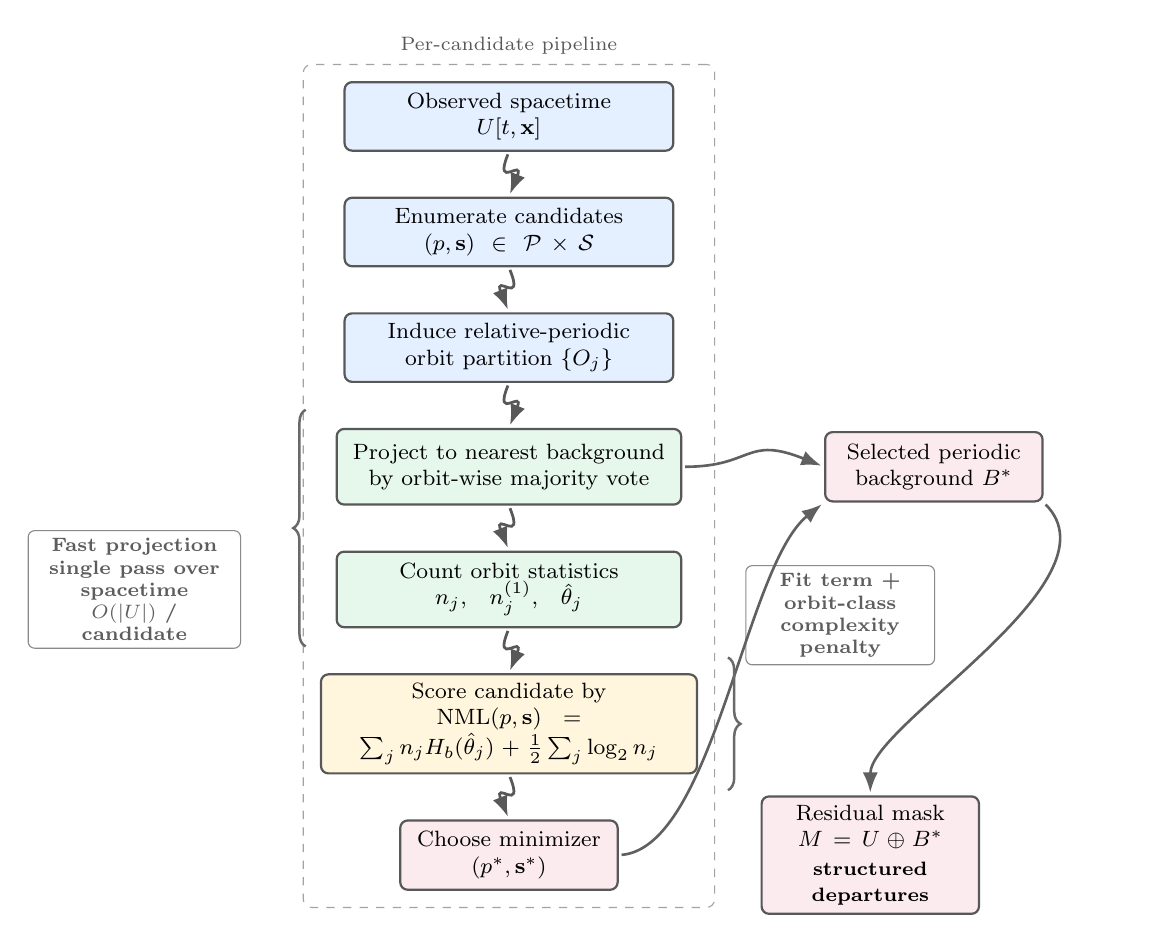
\begin{tikzpicture}[node distance=5.7mm and 8mm]
  % Main pipeline.
  \node[stage] (data) {Observed spacetime\\$U[t,\mathbf{x}]$};
  \node[stage, below=of data] (cand) {Enumerate candidates\\$(p,\mathbf{s}) \in \mathcal{P}\times\mathcal{S}$};
  \node[stage, below=of cand] (orbit) {Induce relative-periodic\\orbit partition $\{O_j\}$};
  \node[compute, below=of orbit] (majority) {Project to nearest background\\by orbit-wise majority vote};
  \node[compute, below=of majority] (stats) {Count orbit statistics\\$n_j,\; n_j^{(1)},\; \hat{\theta}_j$};
  \node[score, below=of stats] (scorebox) {Score candidate by\\$\mathrm{NML}(p,\mathbf{s}) = \sum_j n_j H_b(\hat{\theta}_j) + \tfrac{1}{2}\sum_j \log_2 n_j$};
  \node[output, below=of scorebox] (select) {Choose minimizer\\$(p^*,\mathbf{s}^*)$};

  % Output lane.
  \node[output, right=18mm of majority] (background) {Selected periodic\\background $B^*$};
  \node[output, right=18mm of select] (residual) {Residual mask\\$M = U \oplus B^*$\\[1pt]{\scriptsize\bfseries structured departures}};

  % External notes near the pipeline with explicit scope braces.
  \node[notebox, left=12mm of stats] (fastnote) {Fast projection\\single pass over\\spacetime\\$O(|U|)$ / candidate};
  \node[notebox, above right=1mm and 6mm of scorebox.north east, anchor=south west, text width=22mm] (scorenote) {Fit term +\\orbit-class\\complexity penalty};

  % Main flow with gentle curves rather than straight vertical arrows.
  \draw[flow] (data.south) .. controls +(-2mm,-5mm) and +(2mm,5mm) .. (cand.north);
  \draw[flow] (cand.south) .. controls +(2mm,-5mm) and +(-2mm,5mm) .. (orbit.north);
  \draw[flow] (orbit.south) .. controls +(-2mm,-5mm) and +(2mm,5mm) .. (majority.north);
  \draw[flow] (majority.south) .. controls +(2mm,-5mm) and +(-2mm,5mm) .. (stats.north);
  \draw[flow] (stats.south) .. controls +(-2mm,-5mm) and +(2mm,5mm) .. (scorebox.north);
  \draw[flow] (scorebox.south) .. controls +(2mm,-5mm) and +(-2mm,5mm) .. (select.north);

  % Output flow routed on separate curves.
  \draw[side] (majority.east) .. controls +(9mm,0) and +(-10mm,4mm) .. (background.west);
  \draw[side] (select.east) .. controls +(12mm,1mm) and +(-10mm,-8mm) .. (background.south west);
  \draw[side] (background.south east) .. controls +(10mm,-10mm) and +(0,9mm) .. (residual.north);

  % Braces that show exactly what the notes refer to.
  \draw[decorate, decoration={brace, mirror, amplitude=4.5pt}, line width=0.9pt, draw=linegray!90] ($(majority.north west)+(-3.8mm,2.3mm)$) -- ($(stats.south west)+(-3.8mm,-2.3mm)$);
  \draw[braceann] ($(scorebox.north east)+(3.8mm,2.0mm)$) -- ($(scorebox.south east)+(3.8mm,-2.0mm)$);

  % Group box.
  \begin{scope}[on background layer]
    \node[draw=linegray!55, dashed, rounded corners=3pt, inner sep=6pt,
      fit=(data)(cand)(orbit)(majority)(stats)(scorebox)(select),
      label={[pipelabel]above:Per-candidate pipeline}] {};
  \end{scope}
\end{tikzpicture}
\end{document}
